\documentclass[a4paper, twoside]{article}
\usepackage[utf8]{inputenc} % Especifica la codificación de caracteres de los documentos.
\usepackage[spanish]{babel} % Indica que el documento se escribirá en español.
\usepackage[top=3cm, bottom=2.5cm, inner=1.5cm, outer=2.5cm]{geometry} % Márgenes personalizados
\usepackage{subfiles} % Paquete para incluir el preambulo en los sub archivos.
\usepackage{afterpage} % Permite añadir páginas despues de una página dada.
\usepackage{hyperref} % Permite incluir enlaces en los archivos.
\usepackage{lastpage} % Paquete para poder contabilizar el total de páginas del documento.
\usepackage{fancyhdr} % Permite personalizar los header y footer del documento.
\usepackage{tikz} % Permite incluir los diagramas exportados con DIA
% Defino la ruta de los paquetes personalizados para el apunte

% Matemáticas
\usepackage{amsmath} % para escribir matrices
\usepackage{amsfonts} % \mathbb por ej.
\usepackage{amssymb} % \triangleq por ej. http://ia.wikipedia.org/wiki/Wikipedia:LaTeX_symbols


\newcommand{\rutapaquetes}{./paquetes-apunte}

\usepackage{\rutapaquetes/caratula} % Caratula personalizada (cargada desde caratula.sty)
\usepackage[ocultarrevisores]{\rutapaquetes/colaboradores} % Seccion de colaboradores (cargada y creada con colaboradores.sty)
\usepackage{\rutapaquetes/historial} % Seccion de historial de cambios (cargada y creada con historial.sty)

% Define los estilos de los enlaces interpretados por el paquete hyperref
\hypersetup{
    colorlinks=true,   % false: boxed links; true: colored links
    linkcolor=black,   % color of internal links (change box color with linkbordercolor)
    citecolor=green,   % color of links to bibliography
    filecolor=magenta, % color of file links
    urlcolor=blue,     % color of external links
}

% Define los directorios de las imágenes y gráficos
\graphicspath{ {./} {\rutapaquetes/} {./diagramas/} }

% Define el pagestyle personalizado
\pagestyle{fancy}
\fancyhf{}
\renewcommand{\sectionmark}[1]{\markboth{}{\thesection\ \ #1}}
% Define header para pagina par
\fancyhead[ER]{\rightmark}
% Define header para pagina impar
\fancyhead[OL]{\rightmark}
% Define footer para pagina par
\fancyfoot[EL]{Ejercicios} % Nombre del apunte a la izquierda
\fancyfoot[ER]{Página \thepage\ de \pageref{LastPage}} % Numero de pagina a la derecha
% Define footer para pagina impar
\fancyfoot[OL]{Página \thepage\ de \pageref{LastPage}} % Numero de pagina a la izquierda
\fancyfoot[OR]{Ejercicios} % Nombre del apunte a la derecha

\renewcommand{\footrulewidth}{0.4pt} % Agrego linea que separa el footer

\newcommand{\nombremateria}{75.12 - Análisis Numérico I} % Defino el comando "\nombremateria" para no harcodear el nombre en varios lugares.

% Configura la caratula
\materia{\nombremateria}
\tipoapunte{Apunte Práctico}
\tema{Ejercicios claves}

\begin{document}
% Página en blanco agregada después de la carátula
%\afterpage{
%	\null
%	\thispagestyle{empty}%
%	\addtocounter{page}{-1}%
%	\newpage}
\maketitle % Genera la carátula

\tableofcontents % Genera el índice

\subfile{\rutapaquetes/sobre-el-proyecto.tex} % Inlcuye informacion sobre el proyecto FIUBA Apuntes

% Insertar aquí el contenido del apunte. A continuacion hay secciones a modo de ejemplo.
\newcommand{\e}[1]{\times 10^{#1}}
\section{Errores}

Este es un ejercicio que en el González no está debidamente explicado.

Calcular con tres decimales correctos o significativos la siguiente expresión: $$x=a\, \pi$$ siendo $\bar{a} = 1.3134$.

De acuerdo con lo convenido, asumimos que 1.3134 está correctamente redondeado, por lo tanto su error absoluto inherente es menor o igual que $0.5\e{-4}$.
Por otro lado el problema numérico planteado propagará los errores inherentes de acuerdo a la siguiente expresión:
\[e_x = \pi \, e_{a} + a\, e_{\pi}\]

Tres decimales correctos o significativos significa de acuerdo a la Convención 4.2 que el error absoluto del resultado obtenido debe ser menor o igual, en módulo, a $0.5\e{-3}$; por lo tanto nuestro objetivo es que:

\[ \left| e_x \right| \le 0.5\e{-3} \]

Por la desigualdad triangular:

\[ \left| e_x \right| \le \left| \pi \, e_{a} \right| + \left| a \, e_{\pi}    \right|  \le 0.5\e{-3}  \]

Acoto $\pi \le 3.15$, y $a\le 1.3135$, pues asumo que está bien redondeado (el valor real  $a \in [1.31335; 1.313450)$). Podría también haber usado algo un poco más fino, como $\pi \le 3.1316$ y $a\le 1.313450$, pero dado que estoy estimando una cota no necesito demasiada precisión --más adelante quedará más claro--. En fin:

\[ \left| e_x \right| \le  3.15 \cdot 0.5\e{-4}  +  1.3135\, |e_{\pi}|      \le 0.5\e{-3}  \]

Y despejando: 

\[ \left| e_{\pi} \right| \le  \frac{0.5\e{-3} - 0.5 \e{-4} \cdot 3.15 }{1.3135} \simeq 2.61 \e{-4} \]

Ahora que tenemos esta cota ¿cuántos decimales se necesitan? Necesito la \emph{mínima} cantidad de decimales que me aseguren un error menor o igual a ese. Como uso redondeo, el error es de la forma $e = 0.5\e{-n}$, con $n$ la cantidad de decimales. Dado que $|e_{\pi}| \le 0.261\e{-3}$, podemos acotar:

$$|e_{\pi}| \le 0.5\e{-n} \le 0.261\e{-3}$$

Y despejar entonces: $n\ge4$. Esto mismo se observa en la Figura \ref{fig:g1:errores_cantidad_decimales}.

\begin{figure}
	\centering
	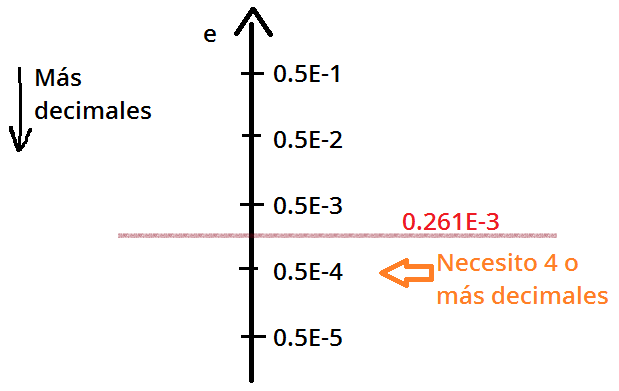
\includegraphics[width=0.4\linewidth]{guia1/errores_cantidad_decimales}
	\caption{Cantidad de decimales y errores inherentes en punto fijo con redondeo.}
	\label{fig:g1:errores_cantidad_decimales}
\end{figure}


De donde deducimos que usando $\pi$ con cuatro decimales significativos y no cometiendo errores apreciables de redondeo en el producto, $\bar{x}$ tendrá tres decimales correctos o significativos, o sea, como:

\[1.3134\cdot 3.1416 = 4.1261774\text{, resulta }x=4.1261774 \pm 0.0005\]

o mejor aún:

\[\bar{x} = 4.126\]



% Bibliografía utilizada en el apunte
\newpage
\newcommand{\bibliographyname}{Bibliografía} % Defino el nombre de la sección de la bibliografía
\addcontentsline{toc}{section}{\bibliographyname} % Agrego la bibliografía en el índice
\renewcommand\refname{\bibliographyname} % Renombro a la bibliografía (por default es 'Referencias')
\begin{thebibliography}{X}
	\bibitem{Cio6} \textsc{John Cioffi}, \textit{ Digital Communication: Signal Processing}, 2013. Course Reader. Chapter 6.  \href{http://www.stanford.edu/group/cioffi/ee379a/}{http://www.stanford.edu/group/cioffi/ee379a/}

\end{thebibliography}


% Incluir los nombres de las personas que han colaborado en la creación del apunte
\colaborador{Fernando Iván Danko (fdanko@fi.uba.ar)}
%\colaborador{Colaborador 2}
%\revisor{}{}
\makeseccioncolaboradores % Crea la seccion de colaboradres

% Incluir el historial de cambios
\revision{22/01/2015}{Versión inicial.}
\revision{29/01/2015}{Agregado ejercicio 5 y cambios estéticos}
\makehistorial

\end{document}